% Prepared for Quantum Information Processing with the Springer Nature
% December 2024 LaTeX template package.
\documentclass[pdflatex,sn-mathphys-num]{sn-jnl}

\usepackage{graphicx}
\usepackage{amsmath,amssymb,amsfonts}
\usepackage{booktabs}
\usepackage{tabularx}
\usepackage{array}
\usepackage{multirow}
\usepackage{url}
\usepackage{xcolor}
\raggedbottom

\begin{document}

\title[Hardware-aware simulation of quantum transfer learning]{Hardware-aware simulation of quantum transfer learning across three visual domains}

\author*[1]{\fnm{Fajri Yanuar Shiddiq} \sur{Juanda}\orcid{https://orcid.org/0009-0007-8894-0265}}\email{fajriyanuar1@gmail.com}
\author[1]{\fnm{Kiki Ahmad} \sur{Baihaqi}\orcid{https://orcid.org/0000-0002-2430-9235}}\email{kikiahmad@ubpkarawang.ac.id}

\affil*[1]{\orgdiv{Department of Informatics Engineering, Faculty of Computer Science}, \orgname{Universitas Buana Perjuangan Karawang}, \orgaddress{\city{Karawang}, \country{Indonesia}}}

\abstract{Statevector evaluations can overstate the operational reliability of variational quantum classifiers. We evaluate a validation-selected quantum transfer-learning head under finite measurement, circuit noise, and restricted connectivity while keeping frozen DINOv2 representations and data splits fixed. Across CIFAR-10, PathMNIST, and EuroSAT, eight-qubit linear circuits retained macro-F1 of 0.9145, 0.7422, and 0.8406 under analytic simulation. At 128 shots, corresponding scores were 0.9137, 0.7397, and 0.8388. Severe synthetic noise mainly damaged calibration and PathMNIST robustness, while topology-aware transpilation avoided up to 60 SWAP gates. The results support resource-aware simulation as a reproducible intermediate step before device execution.}

\keywords{quantum machine learning, variational quantum classifier, finite-shot inference, quantum noise, circuit transpilation, transfer learning}

\maketitle

\section{Introduction}

Variational quantum classifiers are commonly assessed with exact statevectors because analytic expectation values are differentiable and inexpensive at small circuit widths. Such experiments are useful for isolating model behavior, but they omit three constraints that shape execution on gate-based devices. Measurements are estimated from finitely many circuit repetitions, physical gates introduce errors, and a logical interaction graph must be mapped to the available qubit connectivity. A model that performs well under analytic simulation can therefore incur prediction drift, calibration error, or compilation overhead before it reaches a quantum processing unit.

This gap is important for quantum transfer learning. Hybrid pipelines use a classical encoder to reduce image data to a small vector and a parameterized quantum circuit as the predictive head \cite{MARI-2020,PEREZ-SALINAS-2020}. The arrangement makes multi-class visual experiments possible with few qubits, but it also creates several interacting resource choices. Circuit width controls the number of measured observables, circuit depth controls the number of trainable rotations and entanglers, data re-uploading changes the encoding frequency, and the entanglement graph determines both expressivity and routing cost. Expressive circuits may remain difficult to train \cite{MCCLEAN-2018,CEREZO-VQA-2021}, and hardware noise can further flatten optimization landscapes \cite{WANG-NOISE-2021}. Consequently, architecture selection based only on a noiseless test score gives an incomplete account of practical behavior.

Recent studies have strengthened the empirical foundations of quantum machine learning (QML). Work on quantum neural-network capacity, data access, and generalization has shown that favorable model expressivity does not by itself establish a useful advantage \cite{ABBAS-2021,HUANG-2021,CARO-2022,DU-2021,GIL-FUSTER-2024}. Encoding choices define the accessible function class \cite{SCHULD-ENCODING-2021}, while measurement budgets add a separate source of statistical error. Catak formalized this separation through population, empirical, finite-shot, and noisy risk levels \cite{CATAK-2026}. In image classification, Chen compared statevector and shot-based variational models and reported substantial degradation at low shot counts for an amplitude-encoded architecture \cite{CHEN-2024}. These findings motivate experiments that distinguish architecture selection, finite measurement, circuit noise, and compilation rather than treating them as one undifferentiated performance gap.

Noise mitigation and compilation research provides methods for later device studies, including zero-noise extrapolation, probabilistic or symmetry-based mitigation, randomized compiling, and noise-adaptive mapping \cite{TEMME-2017,ENDO-2021,JATTANA-2020,HASHIM-2021,MURALI-2019}. The present study addresses an earlier decision: whether a validation-selected visual VQC remains stable enough under controlled resource perturbations to justify physical execution. This question can be studied without claiming that a simulator reproduces a particular device. Generic depolarizing and readout profiles provide controlled stress levels, and coupling maps expose structural routing overhead. The result is a hardware-aware simulation study rather than hardware validation.

Table~\ref{tab:related} positions the study against adjacent methodological streams. Most visual QML reports emphasize ideal accuracy or a single shot setting. Noise studies often use one task or one architecture, while transpilation studies generally optimize circuits without evaluating predictive stability. We combine these layers in one locked protocol across three visual domains. The same datasets, duplicate-aware partitions, frozen DINOv2 embeddings, six-dimensional learned representation, and training budgets are retained throughout, so the controlled variables are confined to the quantum head and its execution model.

\begin{table}[htbp]
\caption{Related research streams and the unresolved control addressed in this study}\label{tab:related}
\centering
\scriptsize
\setlength{\tabcolsep}{4pt}
\begin{tabularx}{\textwidth}{@{}>{\raggedright\arraybackslash}p{0.19\textwidth}>{\raggedright\arraybackslash}p{0.22\textwidth}>{\raggedright\arraybackslash}p{0.25\textwidth}>{\raggedright\arraybackslash}X@{}}
\toprule
\textbf{Research stream} & \textbf{Representative evidence} & \textbf{Remaining issue} & \textbf{Control used here} \\
\midrule
Hybrid transfer learning & Classical encoder followed by a VQC \cite{MARI-2020,CHEN-2024} & Ideal accuracy does not quantify measurement or hardware constraints & Frozen encoder and representation with separate analytic, shot, noise, and topology evaluations \\
Finite-shot learning & Shot noise affects optimization and empirical risk \cite{KUBLER-2020,SWEKE-2020,CATAK-2026} & Shot effects are often reported for one seed or one task & Four shot budgets, 30 Monte Carlo repetitions, and seed-level bootstrap intervals \\
VQC trainability & Depth and noise can suppress useful gradients \cite{MCCLEAN-2018,WANG-NOISE-2021} & Width, depth, convergence, and predictive quality are rarely reported together & Full 4-by-4 width-depth screen with gradient norms and variances \\
Noise sensitivity & Error mitigation and generic noise models characterize circuit degradation \cite{TEMME-2017,ENDO-2021,JATTANA-2020} & Accuracy alone can hide confidence degradation & Macro-F1, NLL, ECE, Brier score, probability drift, and label flips \\
Hardware mapping & Routing and noise-aware mapping reduce physical overhead \cite{LI-2019,MURALI-2019,HASHIM-2021} & Predictive architecture choice is usually separated from routing cost & Linear and ring logical graphs transpiled to three coupling maps \\
QML benchmarking & Classical data access and preprocessing can dominate outcomes \cite{HUANG-2021,THANASILP-2024,ODAGIU-2025} & Test-driven tuning can inflate evidence & Validation-only selection, frozen hashes, and one post-freeze test evaluation \\
\bottomrule
\end{tabularx}
\end{table}

The study makes four contributions. First, it quantifies how circuit width and depth affect validation performance, optimization time, and gradient statistics. Second, it measures prediction and calibration stability from 128 to 4096 shots over repeated seeds. Third, it separates finite-shot effects from three predeclared circuit-level noise profiles. Fourth, it relates the selected entanglement graph to transpilation depth and SWAP insertion. No result is presented as evidence of quantum advantage, quantum speedup, or performance on a physical device.

\section{Materials and methods}

\subsection{Study design and test isolation}

Figure~\ref{fig:workflow} summarizes the protocol. Architecture screening used CIFAR-10 and PathMNIST because they represent general-object and histopathology images with different class structures. EuroSAT was reserved as a confirmatory remote-sensing domain. All selection decisions used validation macro-F1, with validation negative log-likelihood (NLL) as a tie-breaker. The selected circuit specification and cryptographic hashes of the test manifests were written to an immutable sentinel before test labels could be loaded. The test set was evaluated after this freeze and was not used to revise the selected configurations.

\begin{figure}[htbp]
\centering
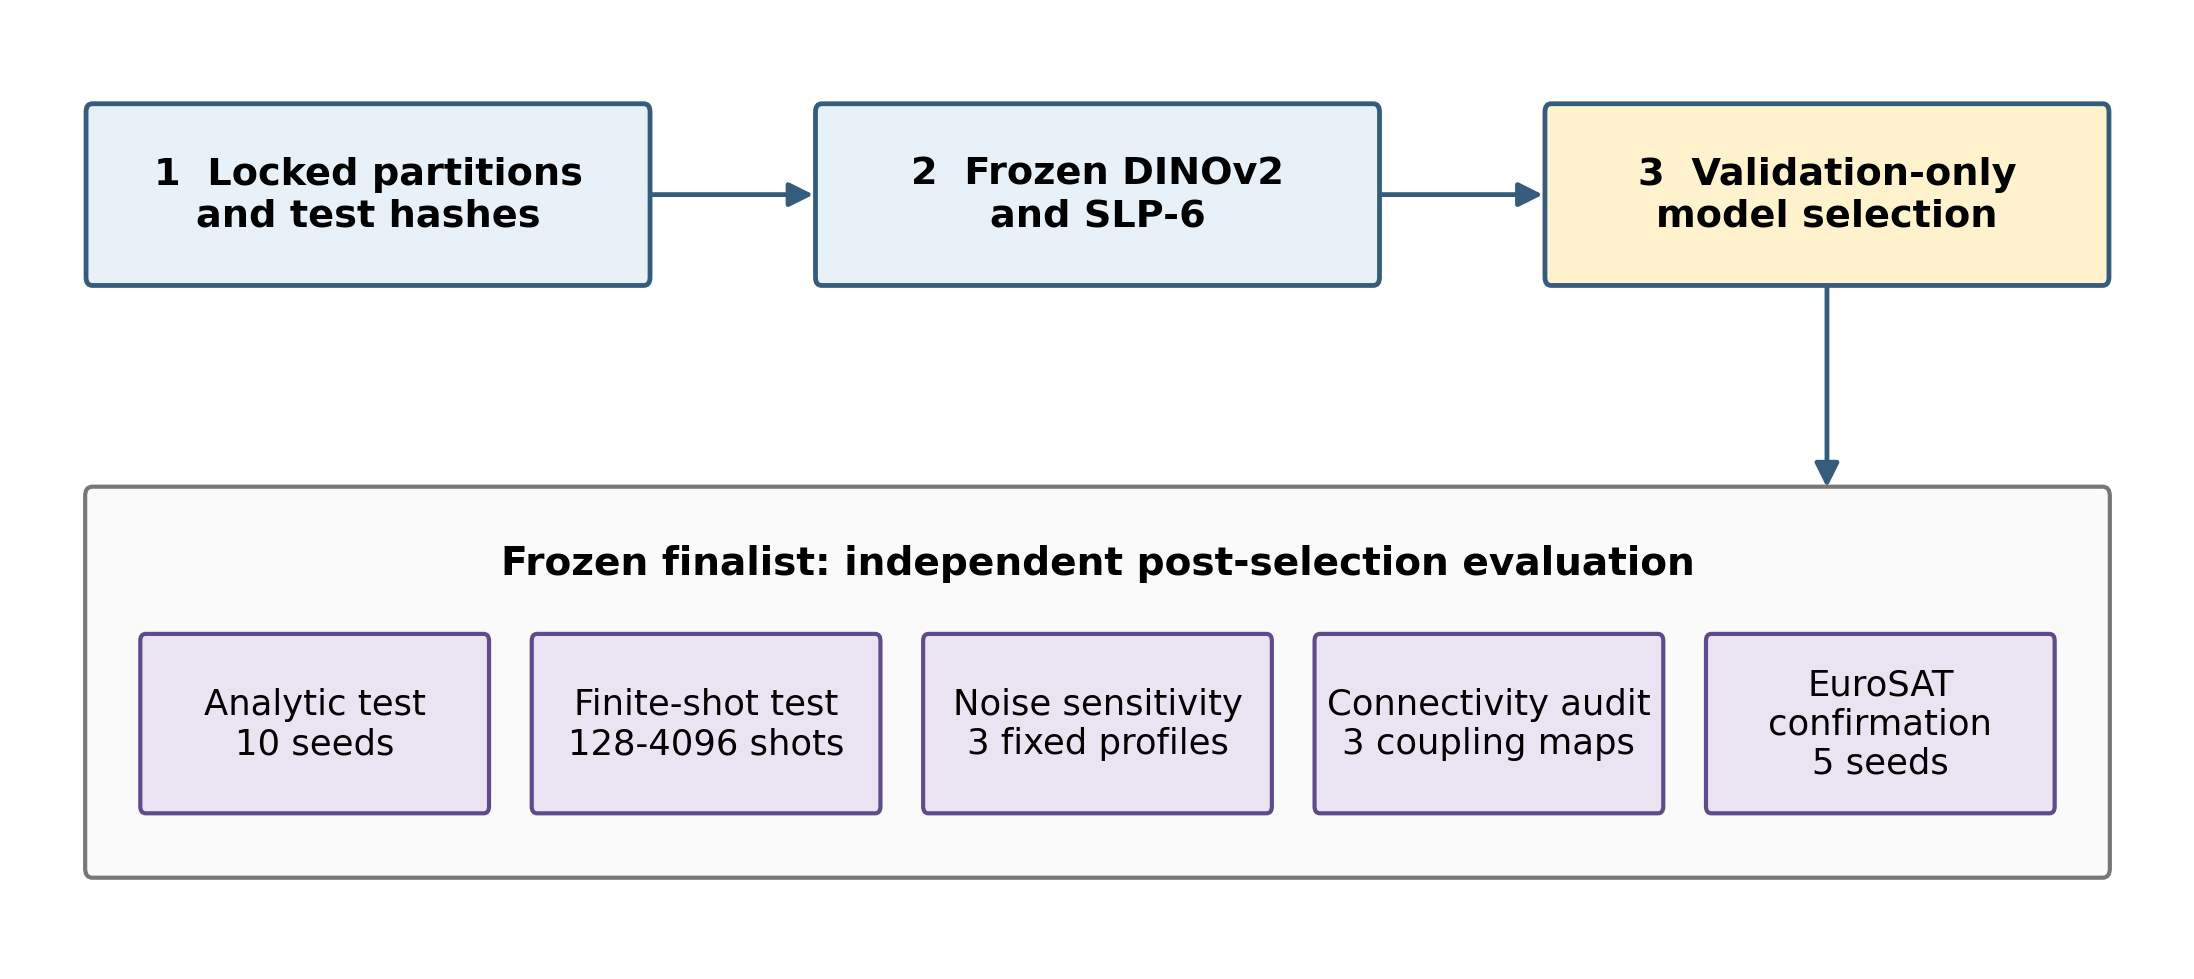
\includegraphics[width=0.98\textwidth]{figures/figure_00_workflow.png}
\caption{Validation-locked experimental workflow from frozen visual representations to analytic, finite-shot, noisy, and connectivity-aware evaluation}\label{fig:workflow}
\end{figure}

The screen crossed 4, 6, 8, and 10 qubits with variational depths 1, 2, 4, and 6. Every screening circuit used one encoding stage and ring entanglement and was trained with five seeds (11, 22, 33, 44, and 55). The two best width-depth pairs per primary dataset entered a factorial ablation of encode-once versus data re-uploading and linear versus ring entanglement. The validation-selected finalist was then trained with ten seeds (11, 22, 33, 44, 55, 66, 77, 88, 99, and 111). EuroSAT compared the common robust finalist with a preregistered six-qubit, depth-two ring reference using five seeds. This staged design limited the search while preserving an independent final evaluation.

\subsection{Datasets and frozen visual representation}

CIFAR-10 contains ten object classes \cite{KRIZHEVSKY-2009}. EuroSAT RGB contains ten land-use and land-cover classes \cite{HELBER-2019}. PathMNIST contains nine colorectal histopathology classes and uses the official MedMNIST splits \cite{MEDMNIST-2023}. Every image was decoded to RGB and audited by exact pixel hash, perceptual hash, and structural similarity. Confirmed duplicate groups were kept within one partition, and cross-split or label-inconsistent groups were quarantined. Table~\ref{tab:data} lists the frozen split sizes.

\begin{table}[htbp]
\caption{Frozen datasets and experimental sample budgets}\label{tab:data}
\centering
\scriptsize
\begin{tabular}{@{}lrrrr@{}}
\toprule
\textbf{Dataset} & \textbf{Classes} & \textbf{Frozen train} & \textbf{Validation} & \textbf{Test} \\
\midrule
CIFAR-10 & 10 & 44,995 & 5,000 & 9,995 \\
EuroSAT & 10 & 18,900 & 4,050 & 4,050 \\
PathMNIST & 9 & 89,991 & 10,001 & 7,179 \\
\bottomrule
\end{tabular}
\end{table}

Each run drew 150 training images per class with a seed-specific stratified sampler. A fixed validation subset used 100 images per class. Images were resized to 224 by 224 pixels, normalized with ImageNet statistics, and passed once through a frozen DINOv2 ViT-S/14 encoder \cite{DINOV2-2024}. The 384-dimensional class token was compressed to six dimensions by a training-fitted single-layer perceptron (SLP-6). The temporary classification layer used to learn this bottleneck was removed. A training-fitted scaler then mapped coordinate $z_j$ to an angle-compatible value

\begin{equation}
x_j = \pi\tanh(z_j), \qquad j=1,\ldots,6.
\label{eq:scale}
\end{equation}

The encoder, reducer, scaler, partitions, and per-seed sample identifiers remained unchanged for every circuit condition. This prevents variation in the classical representation from being mistaken for a circuit effect.

\subsection{Variational quantum classifier}

For a circuit with $q$ qubits and depth $L$, the six scaled features were encoded with $R_Y(x_j)$ rotations. When $q<6$, later features reused wires in sequence; when $q>6$, the additional wires began in $\lvert0\rangle$ and participated through trainable rotations and entanglement. Each variational layer applied a three-parameter rotation to every qubit followed by either a linear CNOT chain or a ring that added a final CNOT from the last qubit to the first. The encode-once circuit can be written

\begin{equation}
U(\boldsymbol{x},\boldsymbol{\theta})=
\prod_{\ell=1}^{L} E_G
\left[\bigotimes_{i=1}^{q}R_Z(\theta_{\ell i3})R_Y(\theta_{\ell i2})R_Z(\theta_{\ell i1})\right]
\left[\prod_{j=1}^{6}R_Y^{(j\bmod q)}(x_j)\right],
\label{eq:circuit}
\end{equation}

where $E_G$ is the CNOT pattern induced by graph $G$. In the re-uploading condition, the encoding product was inserted before every variational layer. The circuit returned marginal Pauli-$Z$ expectation values

\begin{equation}
h_i(\boldsymbol{x})=\langle 0\rvert U^{\dagger}(\boldsymbol{x},\boldsymbol{\theta})Z_iU(\boldsymbol{x},\boldsymbol{\theta})\lvert0\rangle.
\label{eq:expectation}
\end{equation}

A classical linear layer produced $C$ logits, $\boldsymbol{a}=W\boldsymbol{h}+\boldsymbol{b}$, followed by softmax probabilities. The parameter count was $3qL+qC+C$. The selected CIFAR-10 model therefore contained 186 trainable parameters, while the selected PathMNIST and EuroSAT models contained 225 and 234 parameters, respectively.

Training used AdamW with learning rate 0.01, weight decay $10^{-4}$, batch size 32, gradient clipping at 1, a maximum of 100 epochs, and early stopping after 12 unimproved validation epochs. Analytic expectation values and backpropagation were implemented with PennyLane 0.44.1. Training used two NVIDIA GeForce RTX 3080 Ti devices for the cached classical operations and parallel dataset workers; the small statevector circuits themselves were evaluated by the configured simulator backend.

\subsection{Trainability diagnostics}

For each mini-batch $b$, all parameter gradients were flattened into $\boldsymbol{g}_b$. We recorded the Euclidean norm and element-wise variance

\begin{equation}
G_b=\lVert\boldsymbol{g}_b\rVert_2,
\qquad
V_b=\frac{1}{P}\sum_{k=1}^{P}(g_{bk}-\bar g_b)^2,
\label{eq:gradient}
\end{equation}

where $P$ is the number of trainable parameters. Epoch means were stored with every checkpoint. These diagnostics indicate contraction or instability in the observed optimization signal; they are not a formal barren-plateau test because the circuits are small and no asymptotic scaling claim is made.

\subsection{Finite-shot evaluation}

Analytic test probabilities were first computed for every final seed. Because the classifier consumes only marginal Pauli-$Z$ expectations, finite measurement was simulated independently for each marginal. For analytic expectation $h_i$ and shot budget $S$,

\begin{equation}
K_i\sim\operatorname{Binomial}\!\left(S,\frac{1+h_i}{2}\right),
\qquad
\widehat h_i=\frac{2K_i}{S}-1.
\label{eq:shots}
\end{equation}

Shot budgets were 128, 512, 1024, and 4096, with 30 Monte Carlo repetitions per seed and budget. The estimator is exact for the marginal measurement model used by the classifier, but it does not reproduce correlations from a joint bit-string measurement. Seed-level means were formed after averaging repetitions, and 95\% confidence intervals used 10,000 bootstrap resamples of seeds. The expected $S^{-1/2}$ concentration provides the statistical interpretation of increasing the measurement budget \cite{CATAK-2026}.

\subsection{Circuit noise evaluation}

Circuit-level sensitivity was evaluated with Qiskit Aer using depolarizing channels after one- and two-qubit gates and symmetric readout errors. Table~\ref{tab:noiseprofiles} gives the three profiles. Each noisy circuit used 1024 shots and a bidirectional ring coupling map. The experiment used the seed nearest the median validation macro-F1 for each dataset: 99 for CIFAR-10, 33 for PathMNIST, and 55 for EuroSAT. Fixed stratified subsets contained 30 validation and 100 test images per class. These settings make the noise analysis a controlled sensitivity study, not an estimate of variability across seeds or a calibrated model of a named processor.

\begin{table}[htbp]
\caption{Predeclared circuit noise profiles}\label{tab:noiseprofiles}
\centering
\scriptsize
\begin{tabular}{@{}lrrr@{}}
\toprule
\textbf{Profile} & \textbf{One-qubit} & \textbf{Two-qubit} & \textbf{Readout} \\
\midrule
Mild & 0.0005 & 0.005 & 0.01 \\
Medium & 0.0010 & 0.010 & 0.02 \\
High & 0.0020 & 0.020 & 0.04 \\
\bottomrule
\end{tabular}
\end{table}

For each perturbed probability vector $\widehat{\boldsymbol p}_n$ and analytic vector $\boldsymbol p_n$, probability drift was

\begin{equation}
D_p=\frac{1}{NC}\sum_{n=1}^{N}\sum_{c=1}^{C}\left|\widehat p_{nc}-p_{nc}\right|,
\label{eq:drift}
\end{equation}

and label-flip rate was the fraction whose perturbed argmax differed from the analytic prediction.

\subsection{Connectivity-aware transpilation}

Encode-once circuits with both linear and ring logical entanglement were transpiled at optimization level 1 with a fixed transpiler seed. Target coupling maps were all-to-all, bidirectional ring, and bidirectional line. We recorded compiled depth, two-qubit gate count, SWAP count, and total operation count. The audit is structural: it does not contain gate durations or calibration values from a physical backend. It tests whether an architecture's logical interaction graph introduces avoidable routing operations under restricted connectivity \cite{LI-2019,MURALI-2019}.

\subsection{Evaluation measures}

Macro-F1 was the primary endpoint because it weights each class equally. Secondary measures were balanced accuracy, accuracy, Matthews correlation coefficient, macro precision and recall, one-vs-rest macro ROC-AUC, NLL, expected calibration error (ECE) with 15 equal-width bins, and multiclass Brier score \cite{GUO-2017,GNEITING-RAFTERY-2007}. Means and sample standard deviations are reported across independent seeds. Bootstrap intervals are applied only where seed-level replication exists. Noise-profile results are reported descriptively because they use one representative seed.

\section{Results}

\subsection{Width, depth, and architecture selection}

Figure~\ref{fig:scaling} shows the five-seed screen. Increasing depth improved the mean validation macro-F1 until the response flattened or reversed. CIFAR-10 rose from 0.8416 for 8 qubits at depth 1 to 0.9178 at depth 6. PathMNIST rose from 0.6669 to 0.8065 for the same progression. Ten qubits did not improve on eight: at depth 6, CIFAR-10 reached 0.8886 and PathMNIST 0.7654. Width and depth therefore acted as validation-controlled hyperparameters rather than monotonic proxies for quality.

\begin{figure}[htbp]
\centering
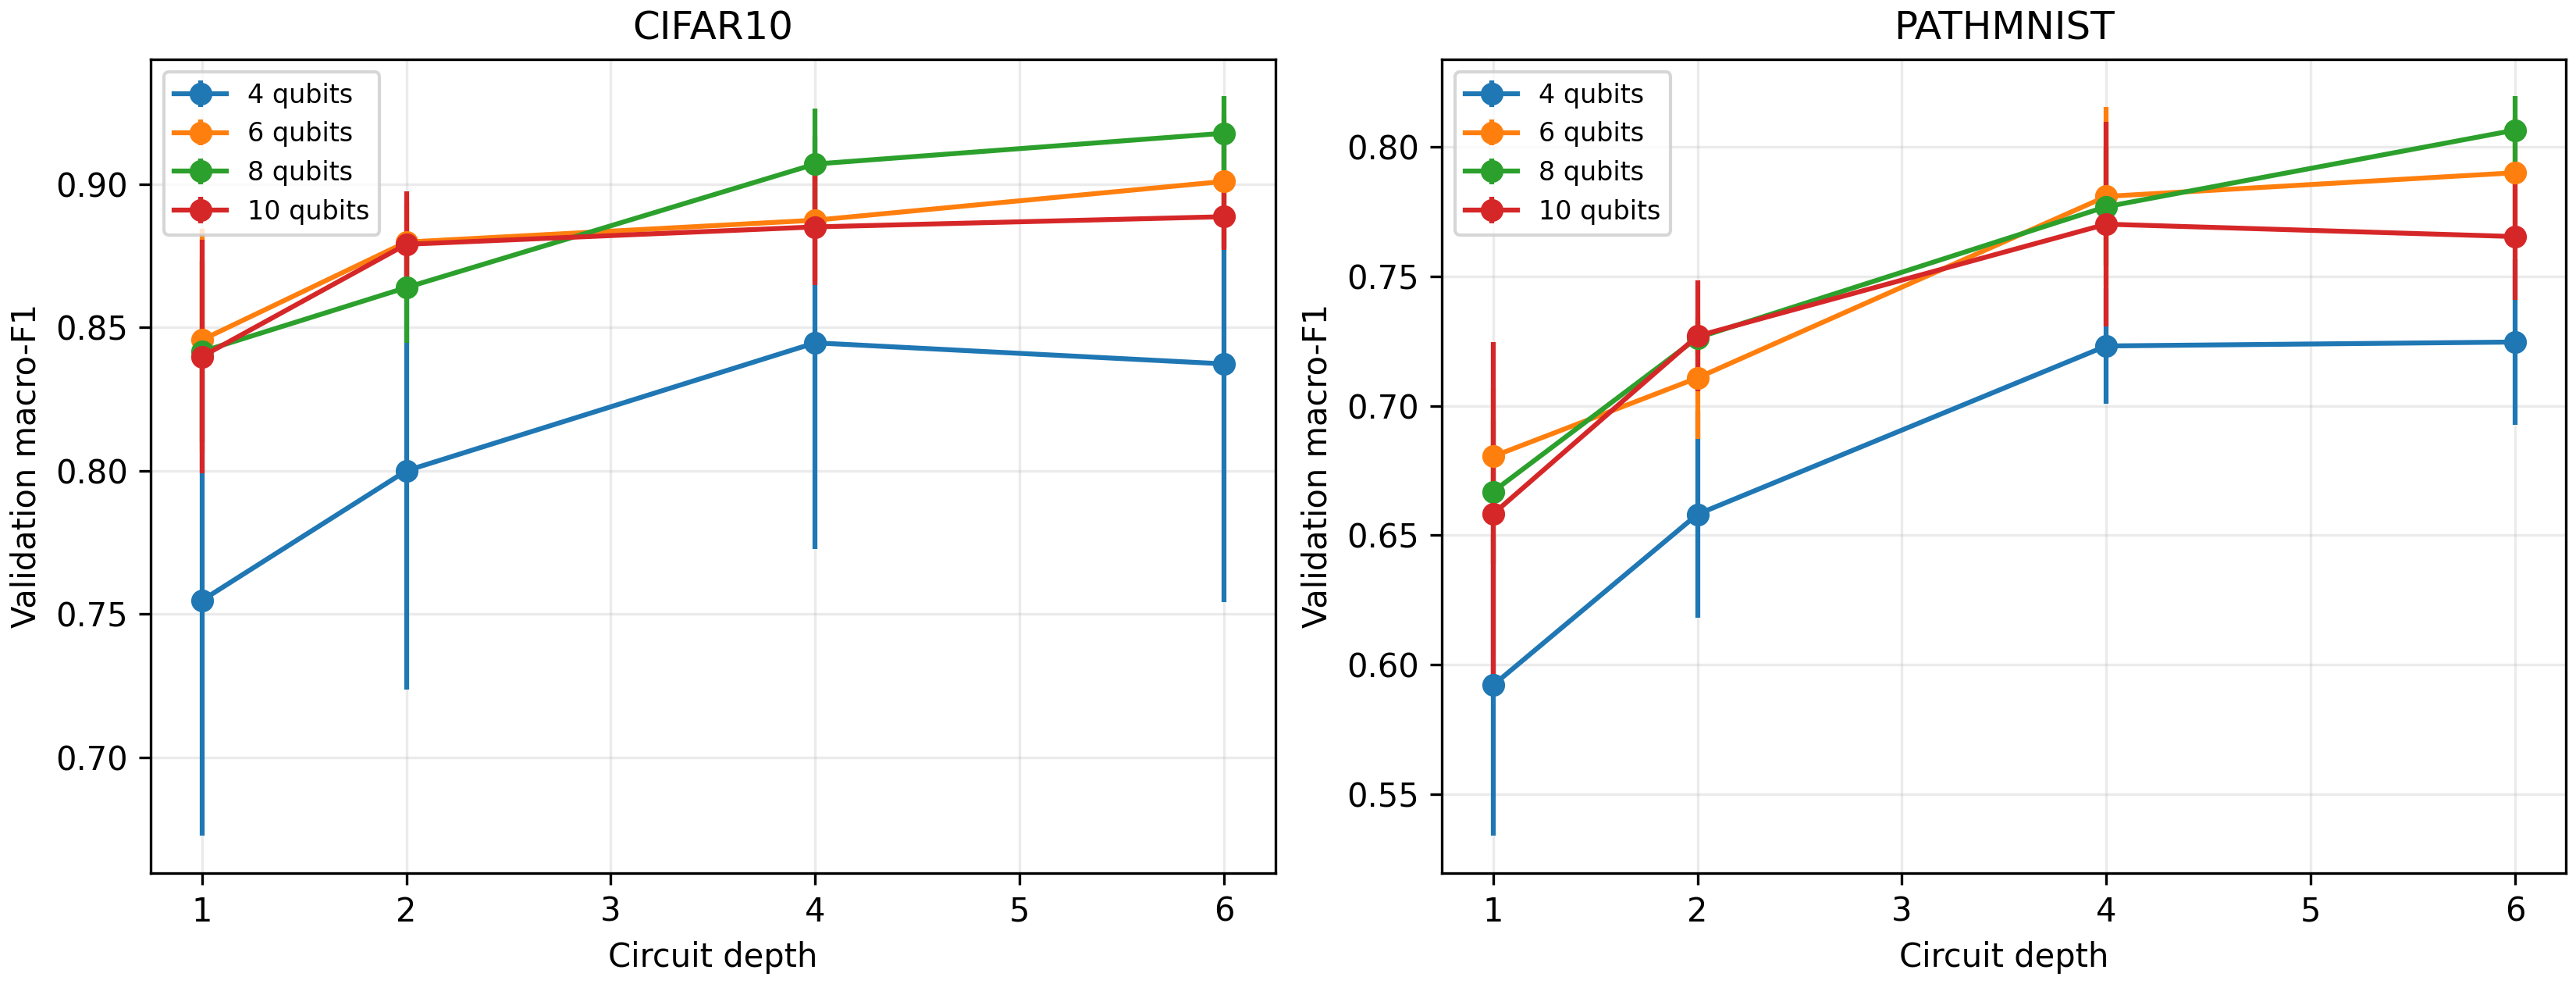
\includegraphics[width=0.98\textwidth]{figures/figure_01_width_depth_scaling.png}
\caption{Validation macro-F1 across circuit width and depth; points show five-seed means and bars show one standard deviation}\label{fig:scaling}
\end{figure}

The encoding and topology ablation favored one encoding stage and linear entanglement. For CIFAR-10 at 8 qubits and depth 4, switching from ring to linear increased validation macro-F1 from 0.9070 to 0.9259. Re-uploading reduced it to 0.8844 with linear and 0.8658 with ring. For PathMNIST at 8 qubits and depth 6, the corresponding scores were 0.8145 for encode-once linear, 0.8065 for encode-once ring, 0.7433 for re-uploaded linear, and 0.6777 for re-uploaded ring. Table~\ref{tab:selected} reports the locked finalists and their confirmatory result.

\begin{table}[htbp]
\caption{Validation-selected configurations and post-freeze analytic test results}\label{tab:selected}
\centering
\scriptsize
\begin{tabular}{@{}lrrrrrrrr@{}}
\toprule
\textbf{Dataset} & \textbf{Qubits} & \textbf{Depth} & \textbf{Encoding} & \textbf{Graph} & \textbf{Seeds} & \textbf{Val macro-F1} & \textbf{Test macro-F1} & \textbf{Test accuracy} \\
\midrule
CIFAR-10 & 8 & 4 & Once & Linear & 10 & $0.9255\pm0.0075$ & $0.9145\pm0.0069$ & $0.9145\pm0.0068$ \\
PathMNIST & 8 & 6 & Once & Linear & 10 & $0.8108\pm0.0117$ & $0.7422\pm0.0283$ & $0.7932\pm0.0232$ \\
EuroSAT & 8 & 6 & Once & Linear & 5 & $0.8501\pm0.0078$ & $0.8406\pm0.0087$ & $0.8452\pm0.0088$ \\
\bottomrule
\end{tabular}
\end{table}

The EuroSAT confirmation was not a new architecture search. Applying the prespecified eight-qubit, depth-six linear circuit improved validation macro-F1 from $0.7672\pm0.0330$ for the six-qubit, depth-two ring reference to $0.8501\pm0.0078$. The smaller standard deviation also indicates that the selected specification transferred more consistently to the third domain.

\subsection{Observed trainability}

Figure~\ref{fig:trainability} summarizes first-epoch gradient variance. The values remained finite for all 32 screened conditions, and every run passed non-finite-gradient checks. The signal nevertheless contracted with width. At depth 6, mean variance decreased from $8.9\times10^{-4}$ at four qubits to $3.2\times10^{-4}$ at ten qubits for CIFAR-10 and from $8.7\times10^{-4}$ to $3.4\times10^{-4}$ for PathMNIST. Ten-qubit training was also slower: CIFAR-10 depth 6 averaged 507.8 s compared with 245.7 s at eight qubits, without a validation gain. These observations support the eight-qubit selection as a performance-compute trade-off but do not establish a barren plateau.

\begin{figure}[htbp]
\centering
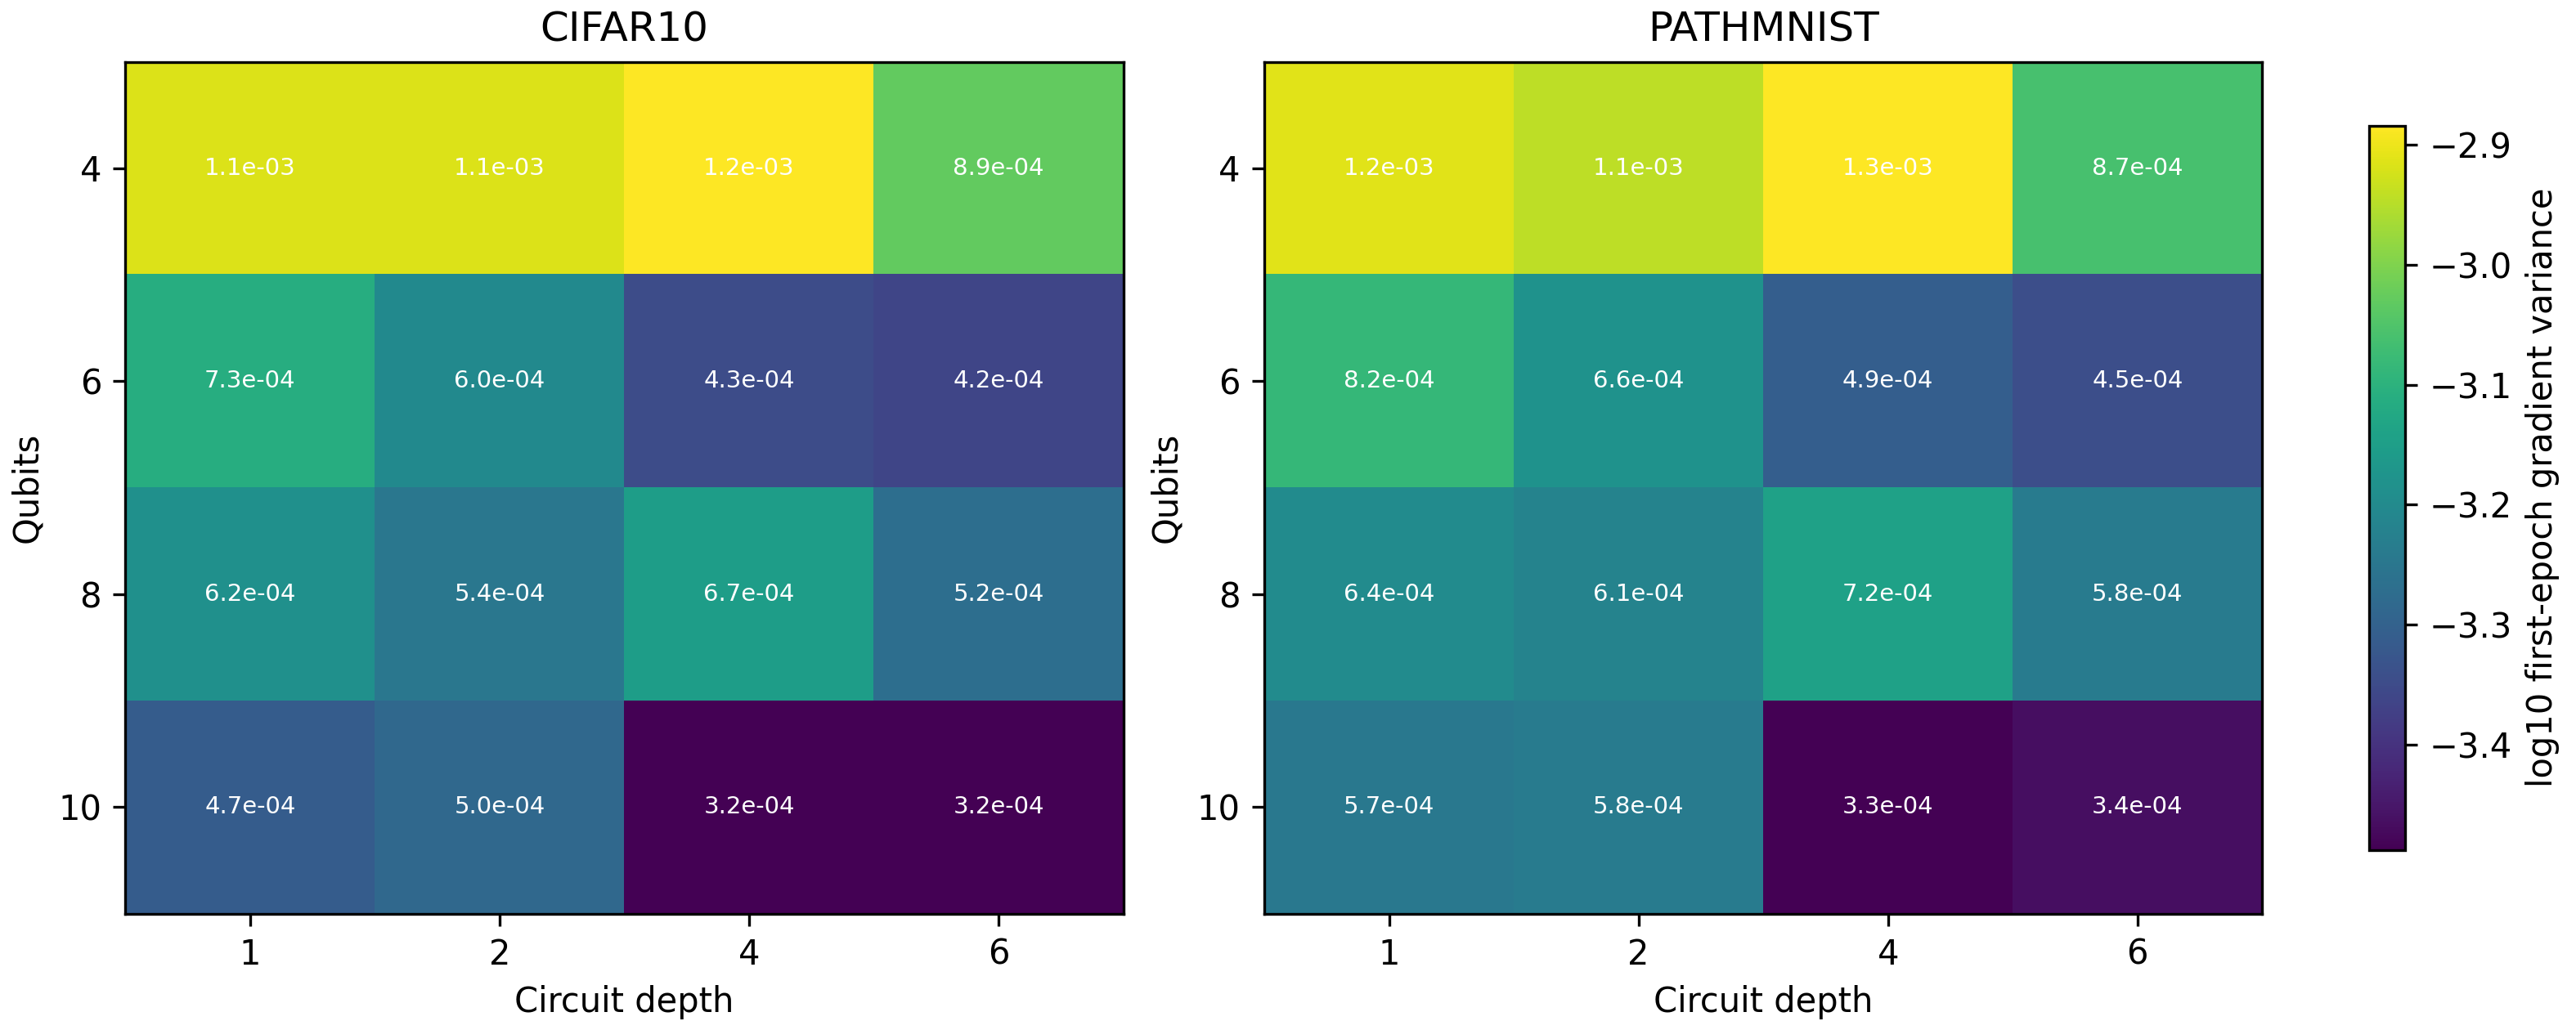
\includegraphics[width=0.98\textwidth]{figures/figure_05_trainability.png}
\caption{Mean first-epoch gradient variance over five seeds for the width-depth screen; cell labels show the untransformed variance}\label{fig:trainability}
\end{figure}

\subsection{Finite-shot stability}

Figure~\ref{fig:shots} and Table~\ref{tab:shots} show that finite measurement caused limited degradation for the selected circuits. CIFAR-10 macro-F1 changed from 0.9145 analytically to 0.9137 at 128 shots. PathMNIST changed from 0.7422 to 0.7397, and EuroSAT from 0.8406 to 0.8388. The corresponding label-flip rates were 0.91\%, 3.15\%, and 2.11\%. Increasing the budget to 4096 shots reduced probability drift and brought all three scores close to their analytic values.

\begin{figure}[htbp]
\centering
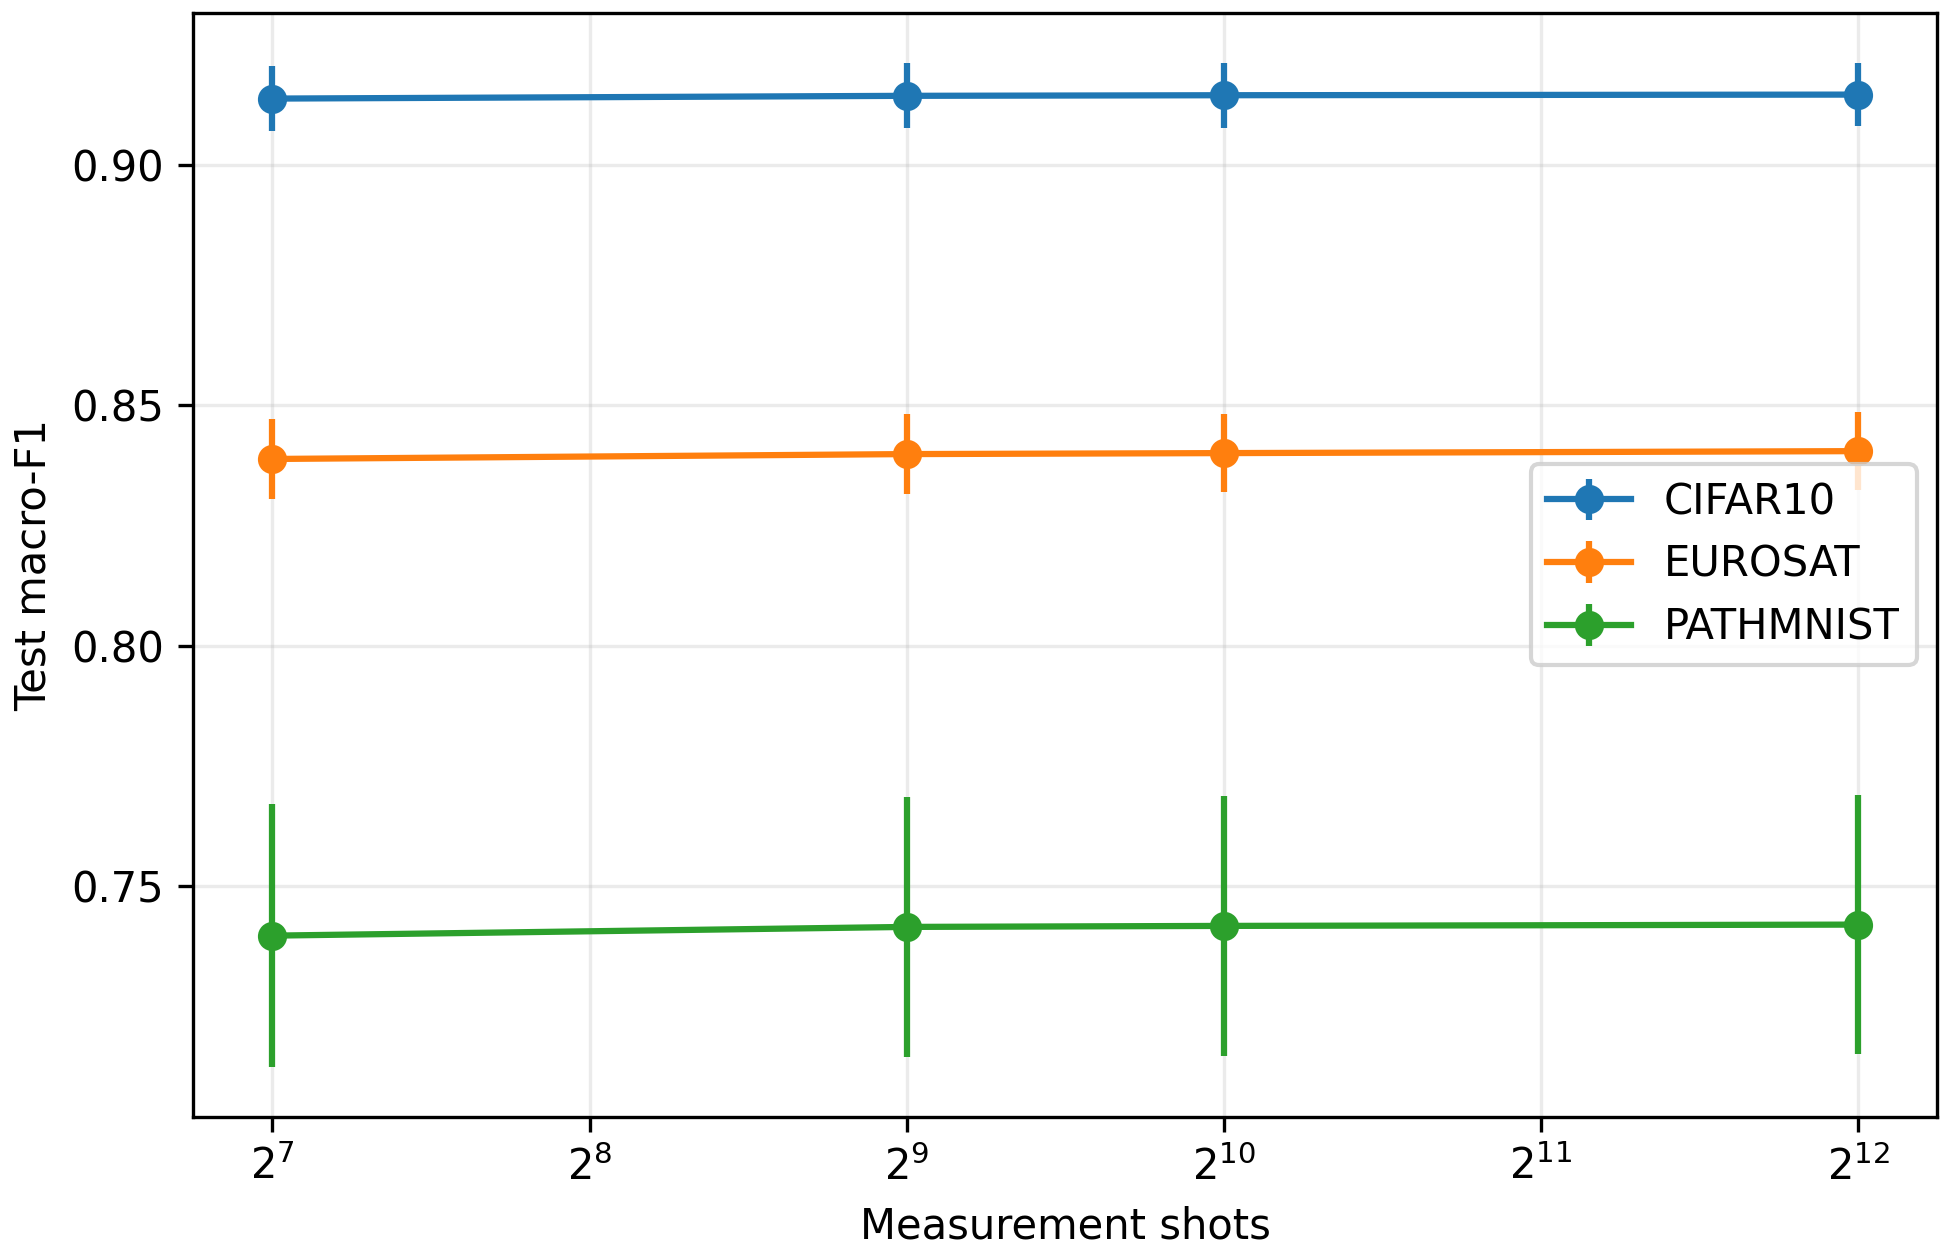
\includegraphics[width=\linewidth]{figures/figure_02_finite_shots.png}
\caption{Test macro-F1 under finite marginal measurement; points are seed means after 30 repetitions and bars show one standard deviation across seeds}\label{fig:shots}
\end{figure}

\begin{table}[htbp]
\caption{Finite-shot test results with 95\% bootstrap intervals for the seed mean}\label{tab:shots}
\centering
\scriptsize
\begin{tabular}{@{}llrrrr@{}}
\toprule
\textbf{Dataset} & \textbf{Shots} & \textbf{Macro-F1 mean} & \textbf{95\% CI} & \textbf{Probability drift} & \textbf{Label flips} \\
\midrule
\multirow{3}{*}{CIFAR-10} & 128 & 0.9137 & [0.9094, 0.9177] & 0.00334 & 0.00905 \\
 & 1024 & 0.9144 & [0.9102, 0.9184] & 0.00113 & 0.00323 \\
 & Analytic & 0.9145 & [0.9104, 0.9184] & 0 & 0 \\
\midrule
\multirow{3}{*}{PathMNIST} & 128 & 0.7397 & [0.7229, 0.7564] & 0.00848 & 0.03147 \\
 & 1024 & 0.7418 & [0.7253, 0.7584] & 0.00293 & 0.01130 \\
 & Analytic & 0.7422 & [0.7250, 0.7588] & 0 & 0 \\
\midrule
\multirow{3}{*}{EuroSAT} & 128 & 0.8388 & [0.8324, 0.8468] & 0.00539 & 0.02110 \\
 & 1024 & 0.8400 & [0.8332, 0.8478] & 0.00186 & 0.00746 \\
 & Analytic & 0.8406 & [0.8337, 0.8481] & 0 & 0 \\
\bottomrule
\end{tabular}
\end{table}

The result differs from reports of large low-shot degradation in other architectures \cite{CHEN-2024}. Our circuit was trained analytically and evaluated by sampling marginal observables after training, whereas shot-based optimization injects measurement noise into every gradient update. The present evidence therefore supports inference stability of the trained head; it does not imply that training the same model with 128-shot gradients would be equally stable.

\subsection{Noise and calibration sensitivity}

Noise affected the three domains differently (Fig.~\ref{fig:noise}). CIFAR-10 macro-F1 remained near 0.905 across all profiles, but ECE increased from 0.0398 analytically to 0.1437 under the high profile. Predictive labels were stable while confidence quality deteriorated. PathMNIST showed the largest class-decision effect: high noise reduced macro-F1 from 0.7632 to 0.7382 and flipped 8.33\% of analytic labels. EuroSAT decreased from 0.8315 to 0.8248 with a 7.30\% label-flip rate. Table~\ref{tab:noise} reports the test subset values.

\begin{figure}[htbp]
\centering
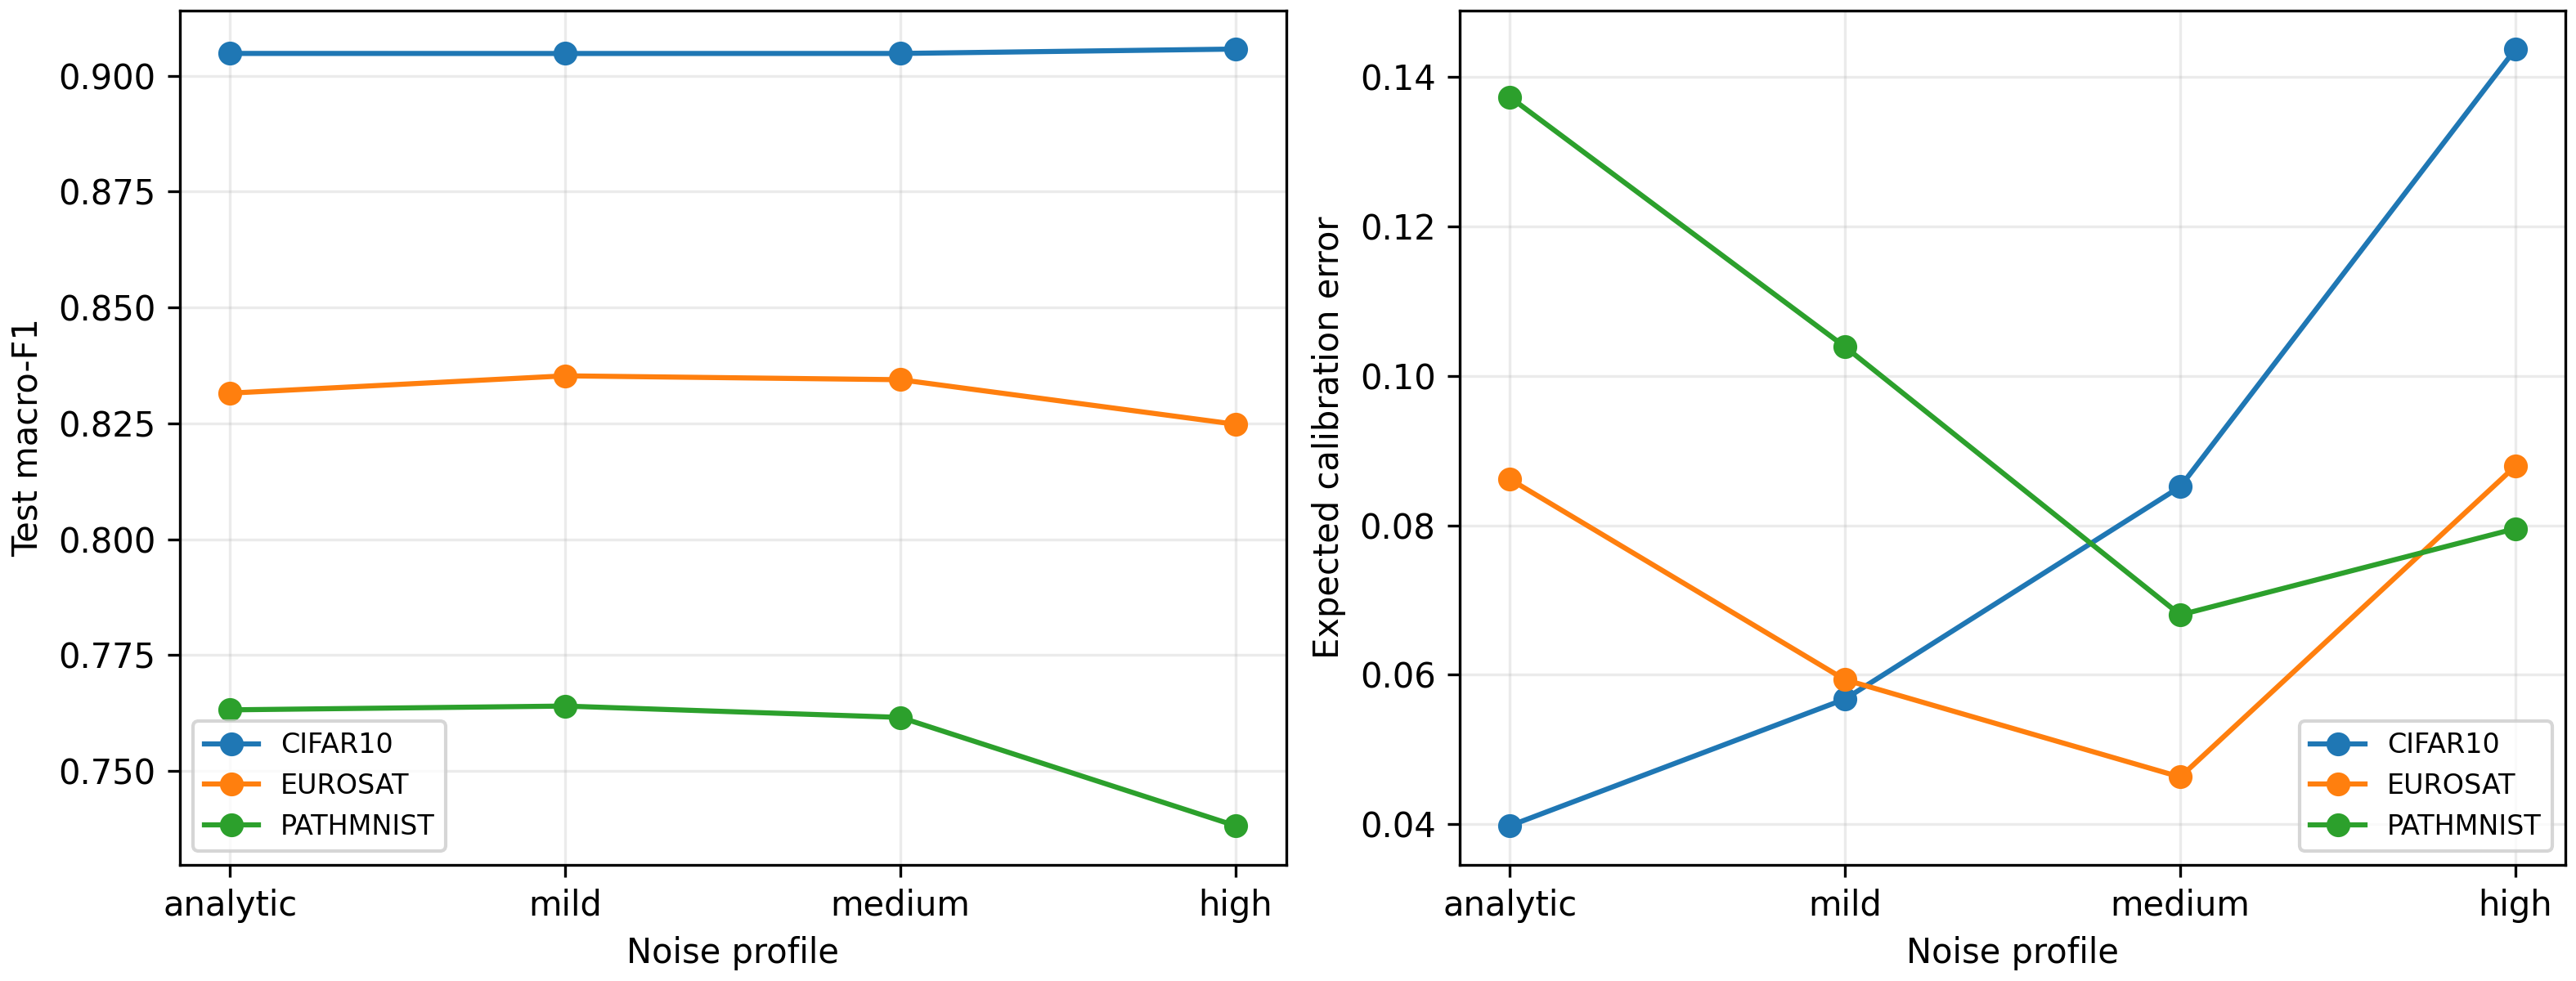
\includegraphics[width=0.98\textwidth]{figures/figure_03_noise_sensitivity.png}
\caption{Macro-F1 and calibration sensitivity under fixed Aer depolarizing and readout profiles; each dataset uses one median-validation seed and a fixed stratified test subset}\label{fig:noise}
\end{figure}

\begin{table}[htbp]
\caption{Circuit-noise sensitivity on fixed stratified test subsets}\label{tab:noise}
\centering
\scriptsize
\begin{tabular}{@{}llrrrrr@{}}
\toprule
\textbf{Dataset} & \textbf{Profile} & \textbf{Macro-F1} & \textbf{NLL} & \textbf{ECE} & \textbf{Probability drift} & \textbf{Label flips} \\
\midrule
\multirow{4}{*}{CIFAR-10} & Analytic & 0.9048 & 0.3928 & 0.0398 & 0 & 0 \\
 & Mild & 0.9048 & 0.3919 & 0.0568 & 0.0052 & 0.0040 \\
 & Medium & 0.9048 & 0.3995 & 0.0852 & 0.0116 & 0.0050 \\
 & High & 0.9057 & 0.4622 & 0.1437 & 0.0291 & 0.0080 \\
\midrule
\multirow{4}{*}{PathMNIST} & Analytic & 0.7632 & 1.1763 & 0.1373 & 0 & 0 \\
 & Mild & 0.7640 & 1.0584 & 0.1039 & 0.0093 & 0.0167 \\
 & Medium & 0.7616 & 0.9857 & 0.0680 & 0.0202 & 0.0344 \\
 & High & 0.7382 & 0.9661 & 0.0796 & 0.0484 & 0.0833 \\
\midrule
\multirow{4}{*}{EuroSAT} & Analytic & 0.8315 & 0.7622 & 0.0862 & 0 & 0 \\
 & Mild & 0.8353 & 0.6998 & 0.0593 & 0.0070 & 0.0160 \\
 & Medium & 0.8344 & 0.6653 & 0.0463 & 0.0150 & 0.0350 \\
 & High & 0.8248 & 0.7066 & 0.0879 & 0.0384 & 0.0730 \\
\bottomrule
\end{tabular}
\end{table}

Some mild and medium profiles lowered NLL or slightly increased macro-F1. These isolated changes should not be interpreted as a beneficial hardware effect. The analysis uses finite stochastic samples, one representative seed, and generic channels; noise can soften overconfident logits while simultaneously moving individual decisions. Probability drift and label flips increase monotonically, providing the more direct evidence of perturbation.

\subsection{Connectivity overhead}

The selected linear entanglement graph maps directly to a line. For eight qubits, depths 1, 2, 4, and 6 required no SWAP gates and compiled to depths 7, 9, 13, and 17. A ring logical graph mapped to the same line required 6, 14, 34, and 60 SWAP gates and compiled to depths 13, 27, 56, and 85 (Fig.~\ref{fig:connectivity}). Thus, the validation-preferred linear graph also avoided routing overhead on the restrictive topology. This alignment was not imposed during model selection.

\begin{figure}[htbp]
\centering
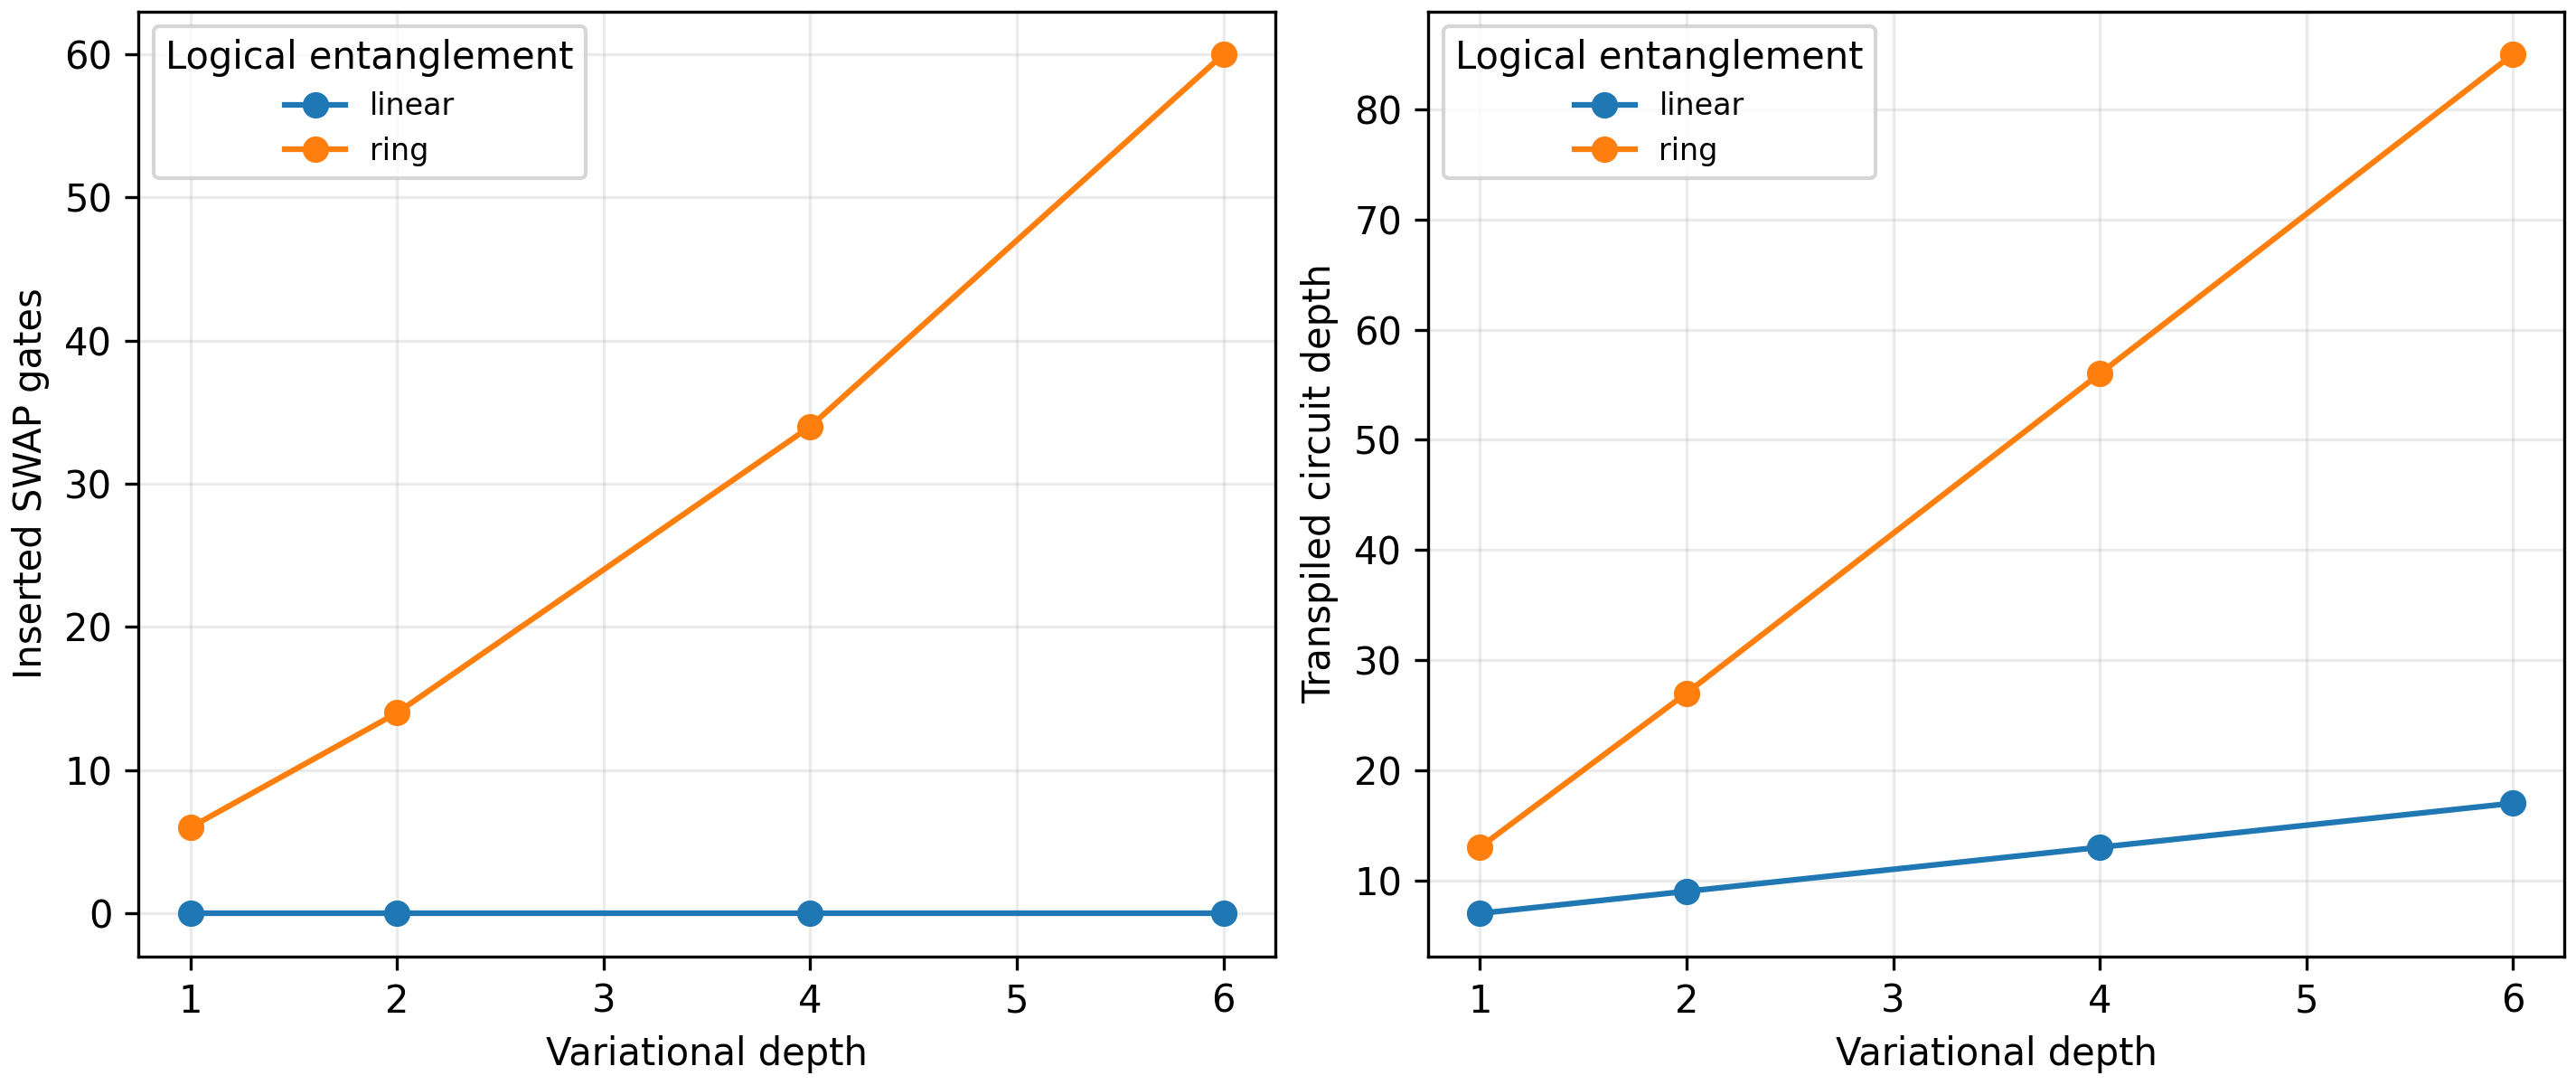
\includegraphics[width=0.94\textwidth]{figures/figure_04_connectivity_overhead.png}
\caption{Routing overhead for eight-qubit encode-once circuits transpiled to a bidirectional line}\label{fig:connectivity}
\end{figure}

The result does not mean that a line is universally preferable. A device with richer coupling may execute a ring without added swaps, and calibrated error rates can outweigh topology alone. It does show that a logical design decision can simultaneously affect validation performance and compilation cost, so reporting the circuit graph without its target connectivity is insufficient for deployment-oriented comparisons.

\section{Discussion}

The main finding is that the validation-selected circuits remained close to their analytic predictive performance under finite marginal measurement, but their behavior under circuit noise was domain- and metric-dependent. At 128 shots, mean macro-F1 decreased by less than 0.0025 in every domain. This stability reflects both the trained decision margins and the fact that measurement noise was introduced only at inference. It should not be generalized to finite-shot training, where gradient estimators require many additional circuit evaluations and can alter convergence \cite{KUBLER-2020,SWEKE-2020}.

The noise experiment adds a complementary result. CIFAR-10 labels were stable even when calibration worsened sharply, whereas PathMNIST and EuroSAT showed more label changes. Accuracy or macro-F1 alone would have missed the CIFAR-10 confidence degradation. This supports reporting proper scoring rules and calibration alongside classification metrics. It also cautions against using a small apparent F1 increase under one stochastic profile as evidence of noise-assisted learning.

Architecture scaling was not monotonic. Eight qubits outperformed ten at the deeper settings, despite the larger circuit's parameter count and runtime. First-epoch gradient variance contracted as width increased, but the observed values remained finite and useful learning occurred. The study therefore avoids labeling the pattern a barren plateau. A formal diagnosis would require controlled initialization ensembles, variance with respect to specific parameters and observables, and wider asymptotic scaling \cite{MCCLEAN-2018,WANG-NOISE-2021}.

The topology ablation produced a practically favorable outcome. Linear entanglement improved validation macro-F1 over the ring for the selected widths and eliminated routing swaps on a line coupling map. This illustrates why hardware-aware design can begin before device access: connectivity is a deterministic constraint that can be audited with a transpiler. It does not replace calibration-aware compilation, which requires a named backend and time-specific error data \cite{MURALI-2019}.

The absence of physical quantum hardware defines the scope of the conclusions. The study demonstrates reproducible sensitivity under finite sampling, declared stochastic channels, and abstract coupling maps. It does not measure queue latency, drift, crosstalk, leakage, non-Markovian errors, or day-to-day recalibration. Generic depolarizing noise cannot reproduce all device-specific failure modes. Similarly, the noise comparison uses one median-validation seed and fixed subsets, so it is a diagnostic stress test rather than a ten-seed estimate. A device study should lock a backend snapshot, transpile against its basis gates and coupling map, repeat jobs across calibration windows, and compare raw with error-mitigated estimates.

The public protocol reduces several risks that remain common in small QML benchmarks. Test manifests were hashed before selection; the same frozen representation was used throughout; every final analytic and shot result retained seed-level replication; and source code, checkpoints, and machine-readable predictions are available. These controls improve auditability but do not establish a quantum advantage. Strong classical alternatives can exploit the same representation, and classical data access remains a central consideration in QML evaluation \cite{HUANG-2021,THANASILP-2024}. The contribution is an execution-sensitivity analysis of a small VQC, not evidence that it surpasses classical computation.

The next experiment should be narrow rather than a repetition of the full architecture search. The locked eight-qubit linear finalists can be executed on a device or a backend-calibrated simulator at one or two shot budgets. Running a stratified subset across several calibration windows would test whether the ranking of domains and the observed calibration sensitivity persist. Error mitigation should be added only after the unmitigated baseline is recorded, preserving a clear comparison between sampling, hardware noise, and mitigation.

\section{Conclusion}

This study followed a validation-selected VQC from analytic simulation to finite measurement, controlled circuit noise, and restricted connectivity. Eight-qubit linear circuits achieved analytic test macro-F1 of 0.9145 on CIFAR-10, 0.7422 on PathMNIST, and 0.8406 on EuroSAT. Finite-shot inference was stable down to 128 shots, while generic circuit noise exposed domain-specific label instability and calibration degradation. Linear entanglement also avoided up to 60 SWAP gates relative to a ring on an eight-qubit line. These results justify hardware-aware simulation as a reproducible screening stage. Physical-device execution remains necessary before making claims about performance on quantum hardware.

\backmatter

\bmhead{Acknowledgments}
The authors received no specific assistance or institutional funding that requires acknowledgment.

\bmhead{Author contributions}
F.Y.S.J. conceived the study, designed the methodology, developed the software, executed and validated the experiments, analyzed the results, prepared the figures, curated the reproducibility package, and wrote the original manuscript. K.A.B. supervised the research, reviewed the experimental design, verified the interpretation, and revised the manuscript. Both authors approved the submitted version.

\bmhead{Funding}
The authors received no funding for this work.

\bmhead{Data availability}
CIFAR-10, EuroSAT, and PathMNIST are publicly available from their original providers. Frozen split manifests, sample identifiers, hashes, and processed experiment tables are available in the project repository at \url{https://github.com/haejoon06/hardware-aware-quantum-transfer-learning}.

\bmhead{Code availability}
Source code, the executed notebook, configuration files, checkpoints, figures, and model archive are available at \url{https://github.com/haejoon06/hardware-aware-quantum-transfer-learning}.

\section*{Declarations}

\bmhead{Ethics approval}
Not applicable. The study used public benchmark datasets and did not involve human participants, identifiable personal data, or animal experiments.

\bmhead{Conflict of interest}
The authors declare that they have no conflict of interest.

\bmhead{Use of generative artificial intelligence}
A generative artificial intelligence tool assisted with manuscript drafting, language editing, and document formatting. The authors verified all numerical claims against the archived outputs and take responsibility for the final content.

\bibliography{references}

\end{document}
